\chapter{First Order Differential Equations}
\section{Linear Equations; Method of Integrating Factors}

\begin{solution}
	\begin{solparts}
		
		\item
		Follows the direction field:
		\begin{figure}[htbp]
			\centering
			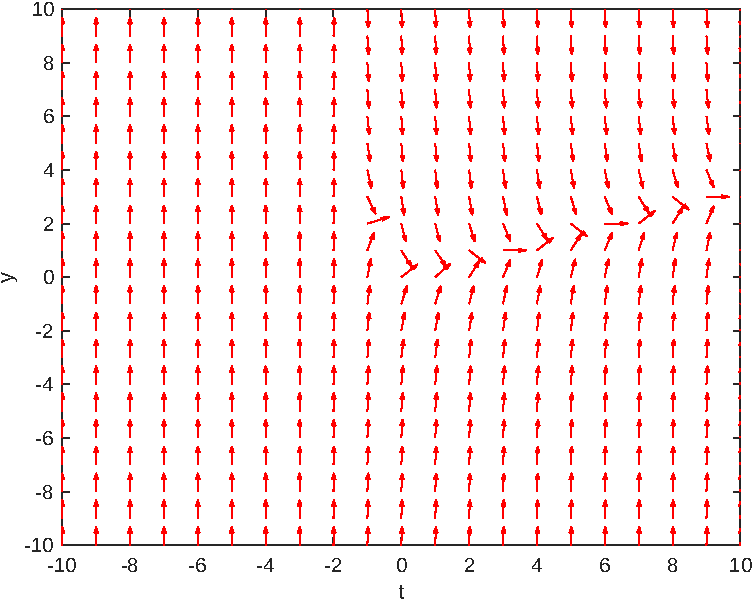
\includegraphics[width=0.5\textwidth]{chapter/img/chapter2/subsection_2.1_1.pdf}
		\end{figure}
	
		\item
		The direction field is governed by the nullcline
		\begin{gather*}
			y(t)=\frac{t+e^{-2t}}{3}.
		\end{gather*}
		As $t\to +\infty$, this curve has asymptotic slope of $\frac{1}{3}$ and separates a lower branch where $y'>0$ from an higher branch where $y'<0$. As $t\to +\infty$ the exponencial term dominates and the field points mostly upward, with the nullcline moving towards very large values of $y$.
		 
		\item 
		\begin{gather*}
			\frac{dy}{dt}+3y=t+e^{-2t}\\
		\end{gather*}
		Using the method os integrating factors, it follows that
		\begin{align*}
			\mu (t)&=e^{\int p(t)\, dt}=e^{\int 3\, dt}\\
			\mu(t)&=e^{3t}.
		\end{align*}
		Thus,
		\begin{gather*}
			\frac{d}{dt}(e^{3t}y)=e^{3t}(t+e^{-2t})\\
			\int \frac{d}{dt}(e^{3t}y)\, dt=\int te^{3t}+t\, dt\\
			y(t)=e^{-3t}\int te^{3t}+t\ dt + ce^{-3t}\\
			y(t)=e^{-3t}(\frac{te^{3t}}{3}-\frac{e^{3t}}{9})+e^{-3t}(e^t)+ce^{-3t}\\
			\boxed{y(t)=\frac{t}{3}-\frac{1}{9}+e^{-2t}+ce^{-3t}}.
		\end{gather*}
	\end{solparts}
\end{solution}

\begin{solution}
	\begin{solparts}
		
		\item
		Follows the direction field:
		\begin{figure}[htbp]
			\centering
			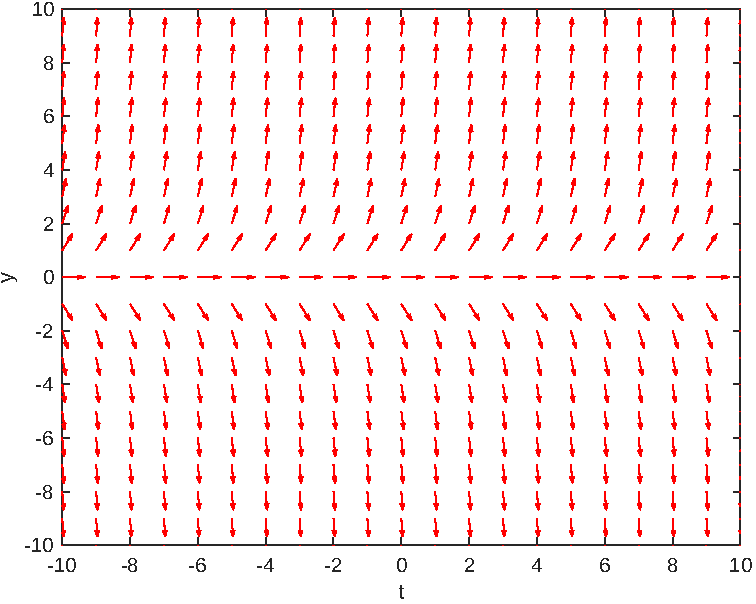
\includegraphics[width=0.5\textwidth]{chapter/img/chapter2/subsection_2.1_2.pdf}
		\end{figure}
	
		\item 
		For any $y$ that remains limited (or grows more slowly than $e^{2t}$), the forcing therm $t^2\, e^{2t}$ dominates when $t\to \infty$. Thus, $f(t,y)\to +\infty$ and the field segments becomes increasingly inclined upwards. Further, the equilibrium solution
		\begin{align*}
			2y+t^2\, e^{2t}&=0,\quad \frac{dy}{dt}=0\\
			y(t)&=0
		\end{align*}
		separates vector with opposite behaviors.
		
		\item 
		\begin{gather*}
			\frac{dy}{dt}-2y=t^2\, e^{2t}
		\end{gather*}
		Using the method of integrating factors, it follows that:
		\begin{align*}
			\mu(t)&=e^{\int p(t)\, dt}=e^{\int -2\, dt}\\
			\mu(t)&=e^{-2t}.
		\end{align*}
		Thus,
		\begin{gather*}
			\frac{d}{dt}(e^{-2t}\, y)=t^2\\
			\int \frac{d}{dt}(e^{-2t}\, y)\, dt=\int t^2\, dt\\
			y(t)=e^{2t}\int t^2\, dt + ce^{2t}\\
			\boxed{y(t)=\frac{t^3}{3}\, e^{2t}+ce^{2t}}.
		\end{gather*}
	\end{solparts}
\end{solution}

\begin{solution}
	\begin{solparts}
		\item
		Follows the direction field:
		\begin{figure}[htbp]
			\centering
			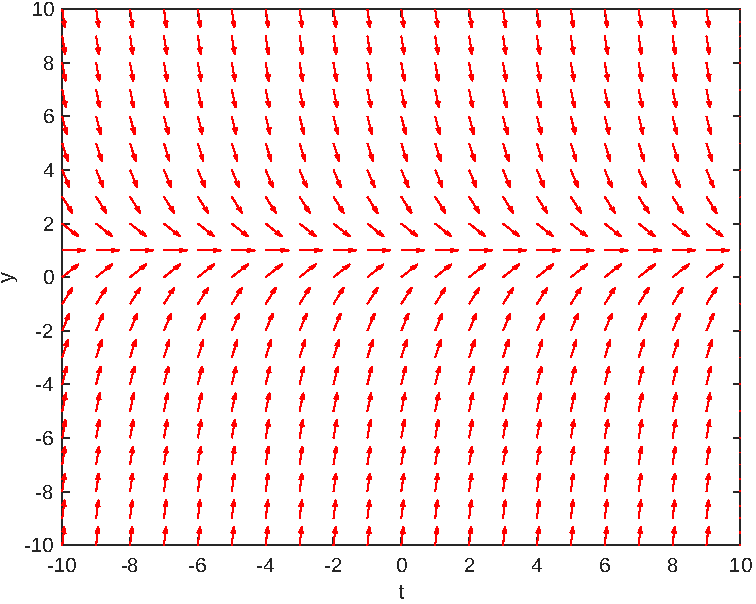
\includegraphics[width=0.5\textwidth]{chapter/img/chapter2/subsection_2.1_3.pdf}
		\end{figure}
	
		\item 
		\textcolor{red}{blablabla}
	
		\item 
		\begin{gather*}
			\frac{dy}{dt}+y=t\, e^{-t}+1
		\end{gather*}
		Using the method of integrating factors, it follows that:
		\begin{align*}
			\mu(t)&=e^{\int p(t)\, dt}=e^{\int dt}\\
			\mu(t)&=e^t
		\end{align*}
		Thus,
		\begin{gather*}
			\frac{d}{dt}(e^t \, y)=t+e^t\\
			\int \frac{d}{dt}(e^t \, y)\, dt=\int t+e^t\, dt\\
			y(t)=e^{-t}\int t+e^t\, dt + ce^{-t}\\
			\boxed{y(t)=e^{-t}\, \frac{t^2}{2}+1+ce^{-t}}.
		\end{gather*}
	\end{solparts}
\end{solution}

\begin{solution}
	\begin{solparts}
		\item
		Follows the direction field:
		\begin{figure}[htbp]
			\centering
			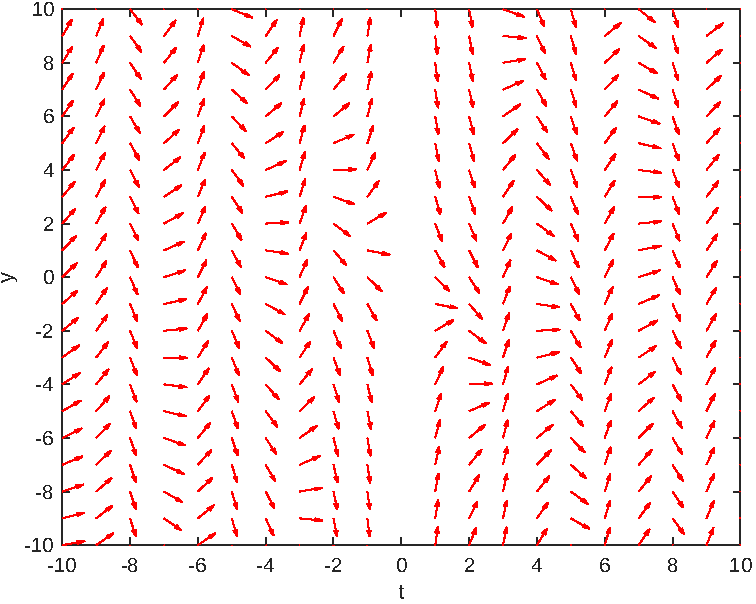
\includegraphics[width=0.5\textwidth]{chapter/img/chapter2/subsection_2.1_4.pdf}
		\end{figure}
	
		\item 
		\textcolor{red}{blablabla}
		
		\item 
		\begin{gather*}
			\frac{dy}{dt}+\frac{y}{t}=3\cos 2t
		\end{gather*}
		Using the method of integrating factors, it follows that:
		\begin{align*}
			\mu(t)&=e^{\int p(t)\, dt}=e^{\int \frac{dt}{t}}\\
			&=e^{\ln |t|}\\
			\mu(t)&=t.
		\end{align*}
		Thus,
		\begin{gather*}
			\frac{d}{dt}(ty)=3t\cos 2t\\
			\int \frac{d}{dt}(ty)\, dt=\int 3t\cos 2t\, dt\\
			y(t)=t^{-1}\int 3t\cos 2t\, dt + ct^{-1}\\
			\boxed{y(t)=\frac{3}{2}\sin 2t +\frac{3}{4}t^{-1}\cos 2t} 
		\end{gather*}
	\end{solparts}
\end{solution}

\begin{solution}
	\begin{solparts}
		\item
		Follows the direction field:
		\begin{figure}[htbp]
			\centering
			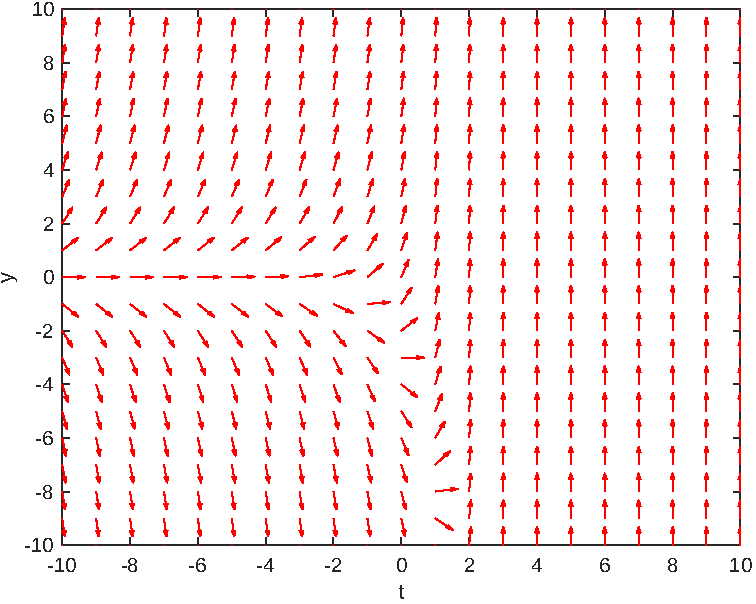
\includegraphics[width=0.5\textwidth]{chapter/img/chapter2/subsection_2.1_5.pdf}
		\end{figure}
		
		\item 
		\textcolor{red}{blablabla}
		
		\item 
		\begin{gather*}
			\frac{dy}{dt}-y=3e^t
		\end{gather*}
		Using the method of integrating factors, it follows that:
		\begin{align*}
			\mu(t)&=e^{\int p(t)\, dt}=e^{-\int dt}\\
			\mu(t)&=e^{-t}
		\end{align*}
		Thus,
		\begin{gather*}
			\frac{d}{dt}(e^{-t}\, y)=3\\
			\int \frac{d}{dt}(e^{-t}\, y)\, dt=\int 3\, dt\\
			y(t)=e^t\int 3\, dt + ce^t\\
			\boxed{y(t)=3t\, e^t + ce^t}
		\end{gather*}
	\end{solparts}
\end{solution}

\begin{solution}
	\begin{solparts}
		\item
		Follows the direction field:
		\begin{figure}[htbp]
			\centering
			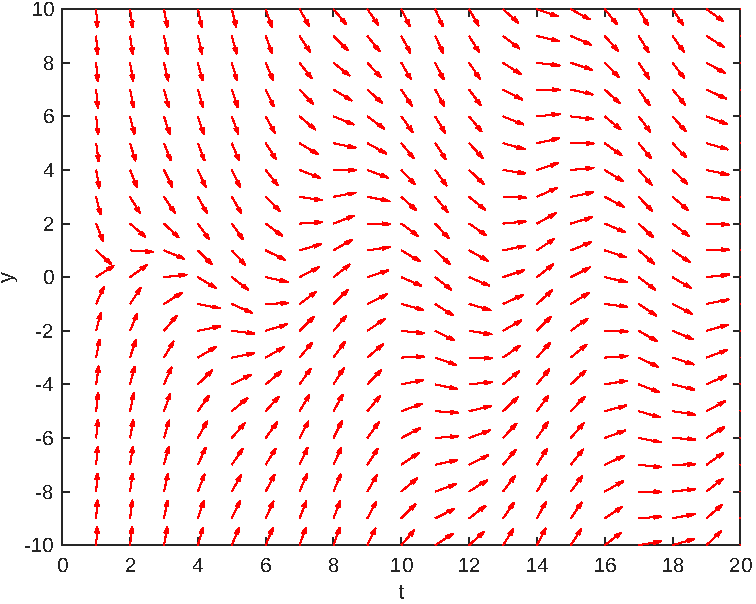
\includegraphics[width=0.5\textwidth]{chapter/img/chapter2/subsection_2.1_6.pdf}
		\end{figure}
	
		\item 
		\textcolor{red}{blablabla}
		
		\item 
		\begin{align*}
			t\frac{dy}{dt}+2y&=\sin t,\quad t>0\\
			\frac{dy}{dt}+2\frac{y}{t}&=\frac{\sin t}{t}
		\end{align*}
		Using the method of integrating factors, it follows that:
		\begin{align*}
			\mu(t)&=e^{\int p(t)\, dt}=e^{\int 2\frac{dt}{t}}\\
			\mu(t)&=t^2
		\end{align*}
		Thus,
		\begin{gather*}
			\frac{d}{dt}(t^2\, y)=t\sin t\\
			\int \frac{d}{dt}(t^2\, y)\, dt=\int t\sin t\, dt\\
			y(t)=t^{-1}\int t\sin t\, dt + ct^{-1}\\
			\boxed{y(t)=-\cos t + t^{-1}\sin t + ct^{-1}}
		\end{gather*}
	\end{solparts}
\end{solution}

\begin{solution}
	\begin{solparts}
		\item 
		Follows the direction field:
		Follows the direction field:
		\begin{figure}[htbp]
			\centering
			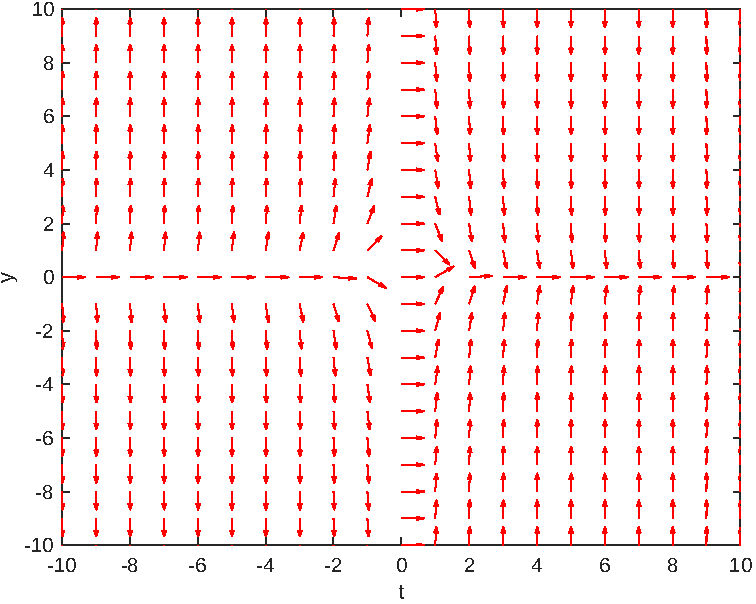
\includegraphics[width=0.5\textwidth]{chapter/img/chapter2/subsection_2.1_7.pdf}
		\end{figure}
	
		\item 
		\textcolor{red}{fsdfdsf}
		
		\item 
		\begin{gather*}
			\frac{dy}{dt}+2ty=2te^{-t^2} 
		\end{gather*}
		Using the method of integrating factors, it follows that:
		\begin{align*}
			\mu(t)&=e^{\int p(t)\, dt}=e^{\int 2t \, dt}\\
			\mu(t)&=e^{t^2}
		\end{align*}
		Thus,
		\begin{gather*}
			\frac{d}{dt}(e^{t^2}y)=2t\\
			\int \frac{d}{dt}(e^{t^2}y)\, dt= \int 2t \, dt\\
			y(t)=e^{-t^2}\int 2t \, dt + ce^{-t^2}\\
			\boxed{y(t)=t^2e^{-t^2}+ce^{-t^2}}
		\end{gather*}
	\end{solparts}
\end{solution}

\begin{solution}
	\begin{solparts}
		
		\item 
		Teste para o problema 21
		\begin{figure}[htbp]
			\centering
			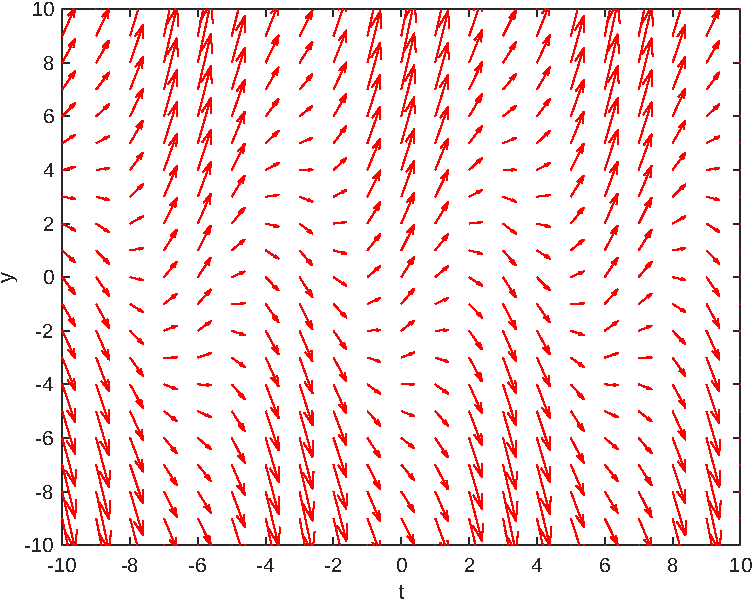
\includegraphics[width=0.5\textwidth]{chapter/img/chapter2/subsection_2.1_21.pdf}
		\end{figure}
	
		\item 
		asdfasd
	\end{solparts}
\end{solution}
\pagebreak
\section{Solutions of Some Differential Equations}
